%%%%%%%%%%%%%%%%%%%%%%%%
%
% $Author: Sadegh Naderi $
% $Datum: 2023-06-30  $
% $Pfad: BA23-02-Sales-Predictor/report/Contents/en/Packages.tex $
% $Version: 1.0 $
% $Reviewed by: Deepti, Sadegh and Raunak $
% $Review Date: 2023-07-1 $
%
%%%%%%%%%%%%%%%%%%%%%%%%




\chapter{Monitoring}


\section{Plan}

The code monitoring plan aims to ensure code quality, identify potential issues, and maintain the overall stability of the software system. This report provides an overview of the code monitoring process.

\begin{itemize}
	\item \textbf{Regular Reviews of the dataframe}: dataframe reviews should be scheduled at defined intervals in the code to assess the quality of the dataframe. 
	
	\item \textbf{Automated Testing}: Automated testing plays a vital role in code monitoring. It involves the use of testing frameworks and tools to execute various types of tests, including unit tests, integration tests, and regression tests.
	
	\item \textbf{Regular Reviews of the code} The code should be thoroughly examined, focusing on aspects such as adherence to coding standards, readability, maintainability, and best practices. Thankfully, Pycharm highlits code style violations for the user, utilizing PEP8 rules 
	
	\item
\end{itemize}



The functions used and the changes in data are explained in the next sections. The code monitoring process for the given code involves monitoring the following steps. :

\begin{enumerate}
	
	\item \textbf{Data loading:} The code begins by loading various datasets using the \texttt{pd.read\_csv()} function. The dataframe \texttt{salesdf} and the transformations of it are the main concern of monitoring.
	
	\item \textbf{Data blending:} The \texttt{process\_sales\_data()} function is used to blend the sales data (\texttt{salesdf}) with other datasets such as \texttt{stores}, \texttt{items}, \texttt{holidays}, and \texttt{oil}. This blending process merges the data based on common columns, such as \texttt{store\_nbr}, \texttt{item\_nbr}, and \texttt{date}, and removes unnecessary columns such as \texttt{description}, \texttt{state}, \texttt{locale\_name}, and \texttt{class}. The merged dataframe will be checked. The data blending and related keys are shown in the Figure \ref{DataBlending}.
	
	\begin{center}
		\begin{figure}[h!]
			\begin{center}
				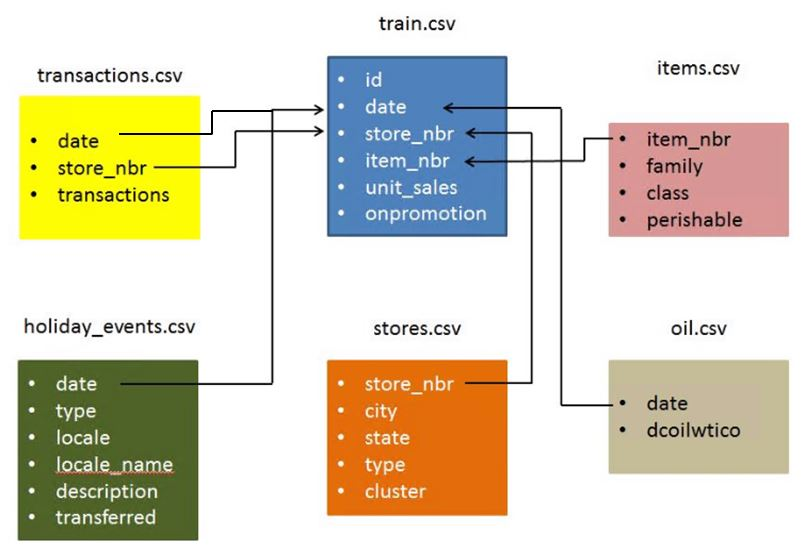
\includegraphics[height=90mm, width=130mm]{Images/DataBlending.jpg}
			\end{center}
			\caption{Data frames and blending with key values \cite{Kaggle:2023}}\label{DataBlending}
		\end{figure}
	\end{center}
	
	\item \textbf{Handling the missing values:} There are subsequent lines of code that modify \texttt{salesdf\_filtered} by filling in missing values for certain columns (\texttt{type\_y}, \texttt{locale}, \texttt{transferred}) with specific values ("no\_holiday" or\\ "no\_locale" in this case). Additionally, rows with missing values in the \texttt{dcoilwtico} column are dropped from \texttt{salesdf\_filtered}. So this process is then monitored by appropriate functions to see if there are any missing values left in the dataframe.
	
	\item \textbf{Data transformation techniques:} Several data transformation techniques are applied in the code:
	\begin{itemize}
		\item \textit{One-Hot Encoding:} Dummy variables are created using the\\ \texttt{pd.get\_dummies()} function for categorical columns such as\\ \texttt{onpromotion}, \texttt{city}, \texttt{type\_x}, \texttt{cluster}, \texttt{store\_nbr}, \texttt{item\_nbr}, \texttt{family}, \texttt{perishable}, \texttt{type\_y}, \texttt{locale}, \texttt{transferred}, \texttt{month}, and \texttt{day}. These dummy variables encode categorical values as binary values (0 or 1) in separate columns.
		\item \textit{Re-scaling:} The \texttt{dcoilwtico} column is re-scaled by subtracting the minimum value and dividing it by the range between the minimum and maximum values. This ensures that the values are normalized within a specific range.
	\end{itemize}
	
	\item \textbf{train-test Splitting:} The \texttt{train\_test\_split()} function from the \\ \texttt{sklearn.model\_selection} module is used to split the transformed data (\texttt{salesdf\_filtered}) into training and testing datasets. The testing dataset size is set to 20\% of the total data (\texttt{num\_test = 0.20}), and a random seed of 15 is used for reproducibility.
	
	\item \textbf{Regression model fitting:} The Code fits an XGBoost regression model (\texttt{XGBRegressor}) using the training data (\texttt{X\_train}) and the corresponding target variable (\texttt{y\_train}). The fitted model is then used to predict the target variable for the testing data (\texttt{X\_test}), and the predictions are stored in the \texttt{y\_pred} variable.
\end{enumerate}




The monitoring process for this code involves reviewing each step for correctness, efficiency, and adherence to coding standards. It is important to ensure that the data loading, blending, filtering, and transformation steps are correctly implemented and that the regression model fitting process is appropriate for the given data and problem. Automated testing is also incorporated into the monitoring process to further enhance code quality and system stability.

\section{Process Description and functions}

The monitoring process involves reviewing each step to ensure correctness, efficiency, and adherence to coding standards:

\begin{enumerate}
	\item \textbf{Data Loading and Shape of Dataframes:}
	\begin{itemize}
		\item Monitor the loading of data from various CSV files (\texttt{stores.csv}, \texttt{items.csv}, \texttt{transactions.csv}, \texttt{oil.csv}, \texttt{holidays\_events.csv}, \texttt{trainnew.csv}) using the \texttt{pd.read\_csv()} function.
		\item Check if the data is correctly loaded into the respective dataframes (\texttt{stores}, \texttt{items}, \texttt{trans}, \texttt{oil}, \texttt{holidays}, \texttt{sales}). This is done using the test functions.
		\item Monitor the shape of each dataframe using the \texttt{shape} attribute and print the shape information. This also, ensures the proper loading of the datasetes
	\end{itemize}
	
	\begin{lstlisting}[language=Python]
		# Monitoring:
		if __name__ == "__main__":
		dataframes = {
			'stores': stores,
			'items': items,
			'trans': trans,
			'oil': oil,
			'holidays': holidays,
			'sales': sales
		}
		
		
		# Monitoring: Print the shape of loaded dataframes
		if __name__ == "__main__":
		for name, df in dataframes.items():
		print("Shape of '{}' dataframe: {}".format(name, df.shape))
		# Monitoring:
		print(sales.info())
	\end{lstlisting}
	
	
	\item \textbf{Monitoring: NA Counts:}
	\begin{itemize}
		\item Iterate over each dataframe in the \texttt{dataframes} dictionary and monitor the presence of missing values (NAs) using the \texttt{isnull().sum()} function.
		\item Print the NA counts for each dataframe if there are any missing values.
	\end{itemize}
	
	\begin{lstlisting}[language=Python]
		# Monitoring:
		if __name__ == "__main__":
		dataframes = {
			'stores': stores,
			'items': items,
			'trans': trans,
			'oil': oil,
			'holidays': holidays,
			'sales': sales
		}
		
		for name, df in dataframes.items():
		na_counts = df.isnull().sum()
		na_columns = na_counts[na_counts > 0]
		if not na_columns.empty:
		print("NA counts for '{}' dataframe:".format(name))
		print(na_columns)
		print()
		# Monitoring:
		if __name__ == "__main__":
		print(salesdf.info())
		print(salesdf.isnull().sum())
		print(salesdf.head(3))
	\end{lstlisting}
	
	
	\item \textbf{Data Blending:}
	\begin{itemize}
		\item Monitor the process of blending the sales data (\texttt{salesdf}) with other dataframes (\texttt{stores}, \texttt{items}, \texttt{holidays}, \texttt{oil}) using the \texttt{merge()} function.
		\item Ensure that the merging is performed correctly based on the specified merge keys 
		\item Again, number of NAs are counted.
		
		\begin{lstlisting}[language=Python]
			# Monitoring:
			if __name__ == "__main__":
			print(salesdf.info())
			print(salesdf.isnull().sum())
			print(salesdf.head(3))
		\end{lstlisting}
		
	\end{itemize}
	
	% ... (continue with the remaining steps)
	
	\item after filtering the data and removing the NA values, the NAs are counted to make sure that the data is cleaned properly
	
	\begin{lstlisting}[language=Python]
		salesdf_filtered['date'] = pd.to_datetime(salesdf_filtered['date'])
		salesdf_filtered['day'] = salesdf_filtered['date'].dt.day_name()
		salesdf_filtered = salesdf_filtered.drop('date', axis=1)
		salesdf_filtered = salesdf_filtered.dropna(subset=['dcoilwtico'])
		
		# Monitoring: count the NAs
		if __name__ == "__main__":
		print(salesdf_filtered.isnull().sum())
	\end{lstlisting}
	
	
	
	after doing the transformation techniques such as re-scaling and one-hot encoding the types of columns are checked and the first 3 rows of the data is viewed for checking the process:
	
	\begin{lstlisting}[language=Python]
		
		# Monitoring:
		if __name__ == "__main__":
		print(salesdf_filtered.dtypes)
		
		# Monitoring:
		if __name__ == "__main__":
		print(salesdf_filtered.head(3))
	\end{lstlisting}
	
	\item Monitoring the model performance
	
	\begin{lstlisting}[language=Python]
		# Monitoring:
		if __name__ == "__main__":
		print('R2 score using XG Boost= ', r2_score(y_test, y_pred), '/ 1.0')
		print('MSE score using XG Boost= ', mean_squared_error(y_test, y_pred), '/ 0.0')
		
		
		plt.plot(y_test.values[:50], '+', color='blue', alpha=0.7, label='True Sales')
		plt.plot(y_pred[:50], 'ro', alpha=0.5, label='Predicted Sales')
		plt.xlabel('Sample Index')
		plt.ylabel('Sales')
		plt.title('True Sales vs Predicted Sales')
		plt.legend()
		plt.savefig('Figure_Output/TrueSalesvsPredicted.png', dpi=300, bbox_inches='tight')
		plt.show()
		
	\end{lstlisting}
	
\end{enumerate}

During the monitoring process, it is important to ensure the proper execution of each step, validate the data consistency and integrity, and verify that any transformations or model fitting procedures are performed accurately. Additionally, logging or saving relevant information and outputs can be useful for future reference and troubleshooting.



\section{New Data and Checking the process}

The only dataframe with NA values is the oil dataframe:

\begin{lstlisting}[language=Python]
	NA counts for 'oil' dataframe:
	dcoilwtico    68
\end{lstlisting}

These are the shapes of the dataframes:

\begin{lstlisting}[language=Python]
	Shape of 'stores' dataframe: (54, 5)
	Shape of 'items' dataframe: (4100, 4)
	Shape of 'trans' dataframe: (83488, 3)
	Shape of 'oil' dataframe: (1218, 2)
	Shape of 'holidays' dataframe: (350, 6)
\end{lstlisting}

This is the salesdf dataframe in its initial state:

\begin{lstlisting}[language=Python]
	id        date  store_nbr  item_nbr  unit_sales onpromotion
	0  125487040  2017-08-15         50    214859         5.0       False
	1  125487041  2017-08-15         50    214860         3.0       False
	2  125487042  2017-08-15         50    215303         5.0       False
\end{lstlisting}

This is the information provided for this dataframe:

\begin{lstlisting}[language=Python]
	RangeIndex: 10000 entries, 0 to 9999
	Data columns (total 6 columns):
	#   Column       Non-Null Count  Dtype  
	---  ------       --------------  -----  
	0   id           10000 non-null  int64  
	1   date         10000 non-null  object 
	2   store_nbr    10000 non-null  int64  
	3   item_nbr     10000 non-null  int64  
	4   unit_sales   10000 non-null  float64
	5   onpromotion  10000 non-null  object 
	dtypes: float64(1), int64(3), object(2)
	memory usage: 468.9+ KB
\end{lstlisting}

after merging the dataframes based on the merging keys, this dataframe would turn into this shape with new columns:

\begin{lstlisting}[language=Python]
	date  store_nbr  item_nbr  ...  locale transferred dcoilwtico
	0  2017-08-15         50    214859  ...   Local       False      47.57
	1  2017-08-15         50    214860  ...   Local       False      47.57
	2  2017-08-15         50    215303  ...   Local       False      47.57
\end{lstlisting}

Since all the columns cannot be printed in the above output, the .column attribute is used to get the columns;

\begin{lstlisting}[language=Python]
	Index(['date', 'store_nbr', 'item_nbr', 'unit_sales', 'onpromotion', 'city',
	'type_x', 'cluster', 'family', 'perishable', 'type_y', 'locale',
	'transferred', 'dcoilwtico']
\end{lstlisting}

The types of columns after one-hot encoding of variables:

\begin{lstlisting}[language=Python]
	unit_sales           float64
	dcoilwtico           float64
	onpromotion_False       bool
	onpromotion_True        bool
	city_Ambato             bool
	...   
	type_y_Holiday          bool
	locale_Local            bool
	transferred_False       bool
	month_08                bool
	day_Tuesday             bool
\end{lstlisting}

The results of the model fitting are shown below:

\begin{lstlisting}[language=Python]
	R2 score using XG Boost=  0.023948033851521555 / 1.0
	MSE score using XG Boost=  0.00010111503764676225 / 0.0
\end{lstlisting}

The Figure \ref{Prediction} shows the comparison of the predicted and real values using the XGBoost model:

\begin{center}
	\begin{figure}[h!]
		\begin{center}
			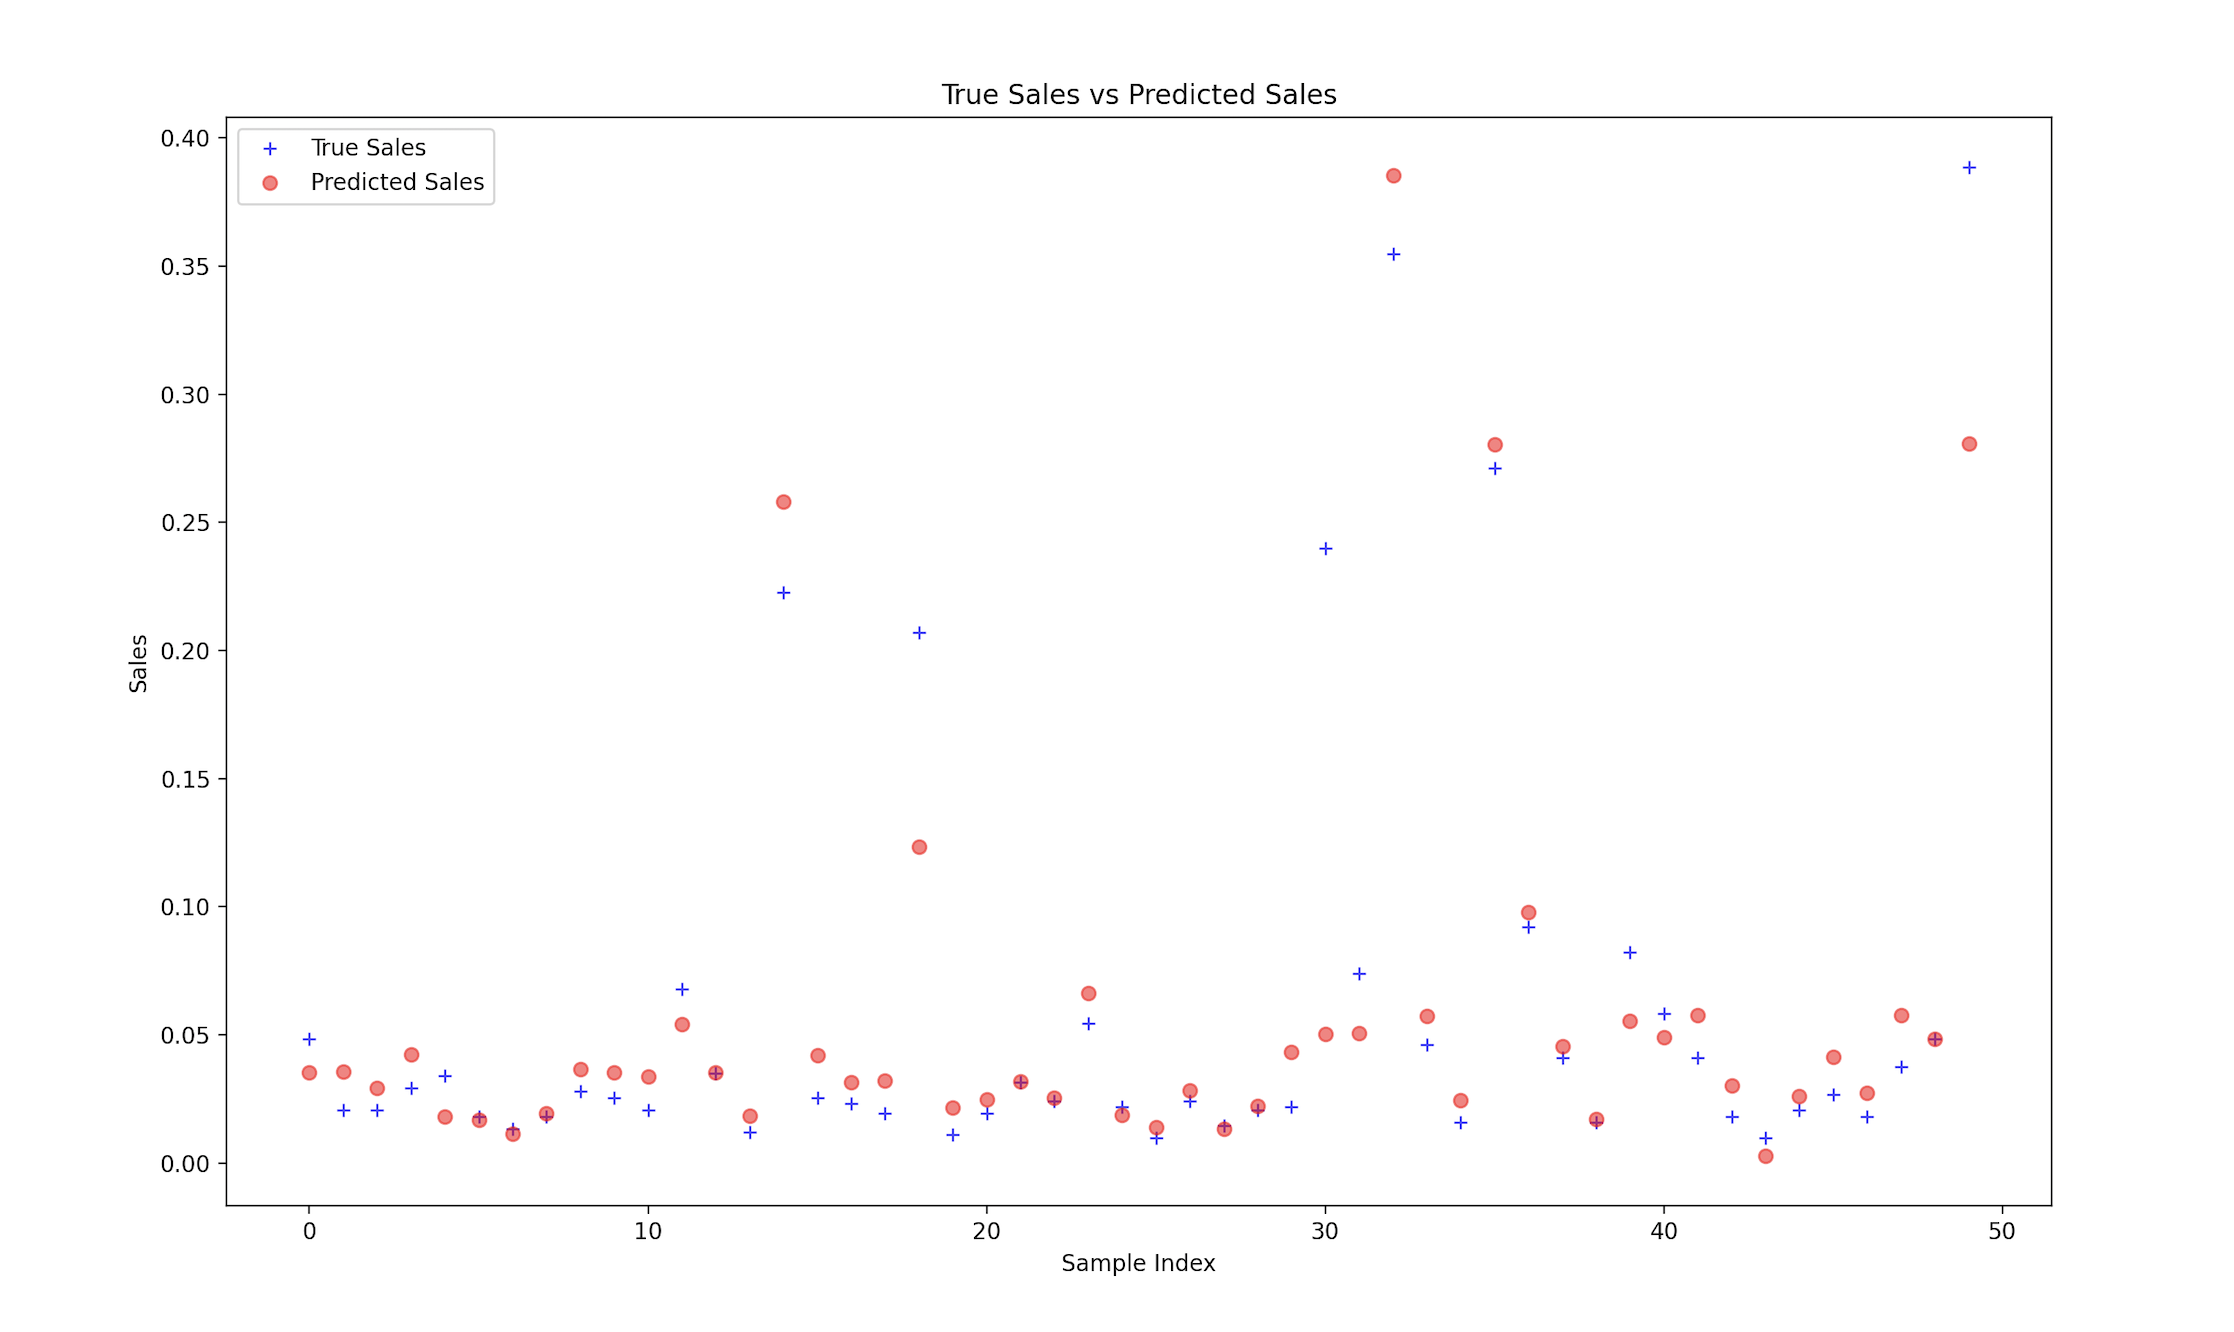
\includegraphics[height=90mm, width=130mm]{Images/Prediction.png}
		\end{center}
		\caption{Comparing predicted and true values}\label{Prediction}
	\end{figure}
\end{center}

\section{Checking the appropriateness of the coding style, PEP8 rules in PyCharm}

PEP8 is a style guide for writing Python code that promotes consistent and readable code. It is utilized in PyCharm. It emphasizes the use of 4-space indentation, limiting lines to 79 characters, employing blank lines for code separation, organizing import statements, following naming conventions, incorporating clear and concise comments, structuring function and method definitions, using whitespace around operators, documenting with docstrings, and maintaining consistency throughout the codebase. Adhering to PEP8 guidelines enhances code readability, maintainability, and collaboration among developers.




	
